\subsection{Isolation Forest}
The goal of this approach is to isolate anomalies from the normal data. The paper \cite{liu2008isolation} describes and evaluates this approach using multiple different data sets.
Based on the hypothesis that anomalies stand out with regard to the values of their attributes, they are identified by the small number of separations necessary to isolate them in the process of recurrent sub-sampling of the data set.

The concept of binary trees is essential for the technique \acfi{IF}.
Every node is either an external or internal node with no or respectively two children. 
Children of a node correspond to a partition of the parent node's data set.

A tree is constructed as follows:
\begin{enumerate}
    \item root of tree $\coloneqq$ data set $X$; $\psi \coloneqq$ sub-sampling size $\widehat{=}$ $|X|$
    \item A parent node $T$, has two children nodes $T_l, T_r$, a test attribute $q$ and a split value $p$
    \begin{enumerate}
        \item $q$ is randomly selected from existing attributes
        \item $p$ is randomly selected within minimum and maximum value of $q$
        \item $T_l \coloneqq \{x \mid x \in X \wedge x[q] < p\}$
        \item $T_r \coloneqq \{x \mid x \in X \wedge x[q] \ge p\}$
    \end{enumerate}
    \item Recursively divide $X$ into sub-samples $X_i$, until either
    \begin{enumerate}
        \item The tree reaches the height limit $l \coloneqq \lceil \log_2 \psi \rceil$
        \item $\vert X_i \vert = 1$
        \item All data in $X_i$ have the same values
    \end{enumerate}    
\end{enumerate}

According to \cite{gruhl2022, liu2008isolation} the characteristics of the constructed trees are:
\begin{enumerate}
    \item $n \coloneqq$ number of external nodes of an \acfi{iTree}
    \item $n-1$ internal nodes in an \ac{iTree}
    \item $h_i(x) \coloneqq $ number of edges from root node to external node $x$ $\widehat{=}$ Path length in \ac{iTree} $i$
    \item $t \coloneqq$ total number of \acp{iTree}
    \item $\bar {h(x)} \coloneqq \frac{1}{t}\sum_{i=1}^{t}h_i(x)$ $\widehat{=}$ average path length of $x$ 
    \item $c(\psi) \coloneqq $ average path length of a binary tree for a given sample set of $\psi$ observations
    \item $s(x, \psi) \coloneqq 2^{-\frac{\bar {h(x)}}{c(\psi)}}$ $\widehat{=}$ anomaly score 
    \begin{enumerate}
        \item $\bar {h(x)} \to c(\psi) \Rightarrow s \to 0.5$
        \item $\bar {h(x)} \to 0 \Rightarrow s(x, \psi) \to 1$ $\widehat{=}$ $x$ is an anomaly
        \item $\bar {h(x)} \to n-1 \Rightarrow s(x, \psi) \to 0$ $\widehat{=}$ $x$ is a normal instance
    \end{enumerate}
\end{enumerate}
%
\begin{figure}
    \begin{subfigure}[t]{0.23\textwidth}
        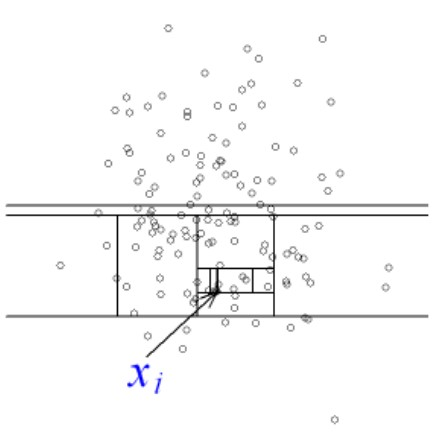
\includegraphics[width=1\textwidth]{images/IF_isolate_normal_inst.jpg}
        \caption{Normal instance}   
        \label{fig:IF_isolate_normal_inst}
    \end{subfigure}
    \begin{subfigure}[t]{0.23\textwidth}
        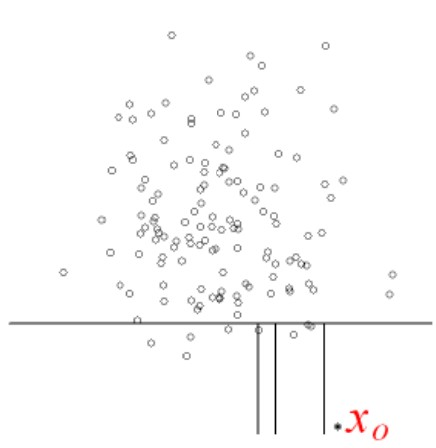
\includegraphics[width=1\textwidth]{images/IF_isolate_abnormal_inst.jpg}
        \caption{Anomaly $x_0$}
        \label{fig:IF_isolate_abnormal_inst}
    \end{subfigure}
    \begin{subfigure}[t]{0.23\textwidth}
        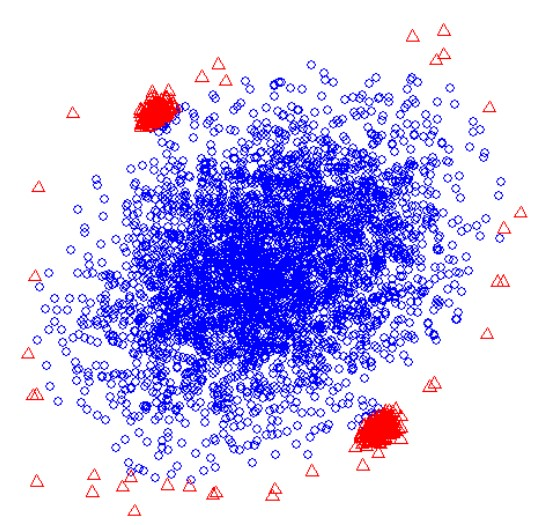
\includegraphics[width=1\textwidth]{images/IF_original_sample.jpg}
        \caption{Original data}   
        \label{fig:IF_original_sample}
    \end{subfigure}
    \begin{subfigure}[t]{0.23\textwidth}
        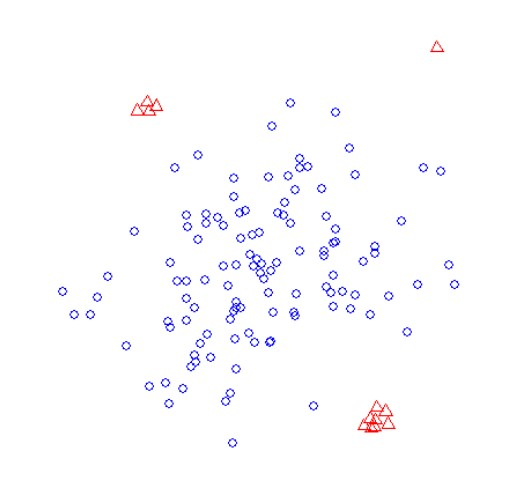
\includegraphics[width=1\textwidth]{images/IF_subsample.jpg}
        \caption{Sub-sample}
        \label{fig:IF_subsample}
    \end{subfigure}
    \caption{Visualisation of instance isolation and sub-sampling from \cite{liu2008isolation}. 
    The normal instance $x_i$ in \autoref{fig:IF_isolate_normal_inst} requires more partitions (visualised by horizontal and vertical lines) to be isolated than the anomaly $x_0$ in \autoref{fig:IF_isolate_abnormal_inst}, due to $x_0$'s solitary position.
    In \autoref{fig:IF_original_sample} for the original data and \autoref{fig:IF_subsample} for a sub-sample of the original data, blue circles denote normal instances, whereas red triangles denote anomalies. Anomalies are isolated quicker in less dense data sets such as \autoref{fig:IF_subsample}.}
\end{figure}
%
The approach is based on the hypothesis, that anomalies are less frequent (a minority in the data set) and have attribute values that extremely deviate from those of normal instances. 
Based on this hypothesis, the authors of \cite{liu2008isolation} conclude, that anomalies, as depicted in \autoref{fig:IF_isolate_abnormal_inst}, require fewer partitions to be isolated than normal instances of a data set, which is visualised in \autoref{fig:IF_isolate_normal_inst}. 
The number of partitions required to isolate a data point is equal to path length $h_i(x)$ in an \ac{iTree} $i$. 
Hence, an average path length of $\bar {h(x)} \to 0$ suggests that the grand majority of the \acp{iTree} has short paths from the root to the instance $x$ and thus, consider $x$ an anomaly.

Anomalies are identified as nodes having shorter path lengths, which means they are isolated earlier than normal instances. 
Hence, the process of dividing the data set into sub-samples can be terminated at the tree height limit $l$, since the anomalies should be isolated by then. 
However, not all normal instances are isolated at this point and thus, a partial model is created.
If a data point $x$ belongs to the part of the tree, which was not built, because for instance, the tree height limit $l$ has been reached and thus, expansion was terminated, an adjustment account $c(\text{size of unbuilt subtree})$ is added when calculating its path length.

Since \acp{iTree} work well if the sampling size is kept small, sub-sampling is conducted. Comparing \autoref{fig:IF_original_sample} and \autoref{fig:IF_subsample}, it becomes clear that fewer data points are favourable to the isolation technique since they are less dense and thus, anomalies are more likely to be isolated early.

According to \cite{liu2008isolation}, swamping refers to wrongly identifying normal instances as anomalies. Masking is the existence of too many anomalies concealing their own presence. Both problems arise from too much data. \acp{iTree} build a partial model by sub-sampling and thus, control the data size and specify on a sub-sample of anomalies or respectively a lack of them. 

Anomaly detection using \acp{IF} is a two-stage process. 
As stated in \cite{gruhl2022, liu2008isolation}, first, in the training stage, sub-samples of size $\psi$ from the training set are used to build \acp{iTree}. 
Then, in the evaluation stage, test instances are passed through the \acp{iTree} to obtain anomaly scores based on their path length. 
The highest $m$ anomaly scores correspond to the $m$ anomalies identified by the \ac{IF}. 

The input parameter $\psi$ controls the input data size in the training stage whereas the number of trees $t$ controls the ensemble size. 
Empirical studies from \cite{liu2008isolation} suggest that $\psi = 2^8 = 256$ and $t = 100$ are optimal to perform anomaly detection across a wide range of data.
Owing to the fact that there are multiple \acp{iTree} it is called a forest. 
Obviously, multiple \acp{iTree} have different sets of partitions, due to the fact that they are randomly generated.